
\section{\label{sec:PerformanceEvaluation}Performance Evaluation}

There are at least three main reasons for having performance evaluations:
\begin{itemize}
\item To review the system with respect to its performance goals
\item To compare the performance of two or more similar systems
\item To find bottlenecks
\end{itemize}
The investigations are implemented in more details, as described in
this section. In order to get a good balance between testing systematically,
and testing with realistic data, we have used two data models in the
testing phase.
\begin{itemize}
\item The \emph{Diving School} model. This data model represents a realistic
data model, i.e. a model that would realistically appear in a small
business setting.

\begin{itemize}
\item Defines the kinds: Person, Student (extending Person), Teacher (extending
Person), CourseType and Course.
\item Defines relations for describing course dependency, student enrollment
on courses, passed courses for students, assigned teachers on courses,
and teaching abilities on course types.
\end{itemize}
\item The \emph{Test Model}: This data model is a more systematically build
data model.

\begin{itemize}
\item Defines the kinds: TestKindNoAttributes, TestKindOneAttribute, TestKindTwoAttributes,
TestKindThreeAttributes, etc. Each kind has the number of attributes
that its name describes -- the attribute is of type PosInt (a positive
integer).
\end{itemize}
\end{itemize}
Having the diving school model means that we can come up with tests
that are realistic, which can be easier to design than systematically
and comprehensively testing a long series of possible data model compositions.

However, it is also interesting to systematically measure how much
data can actually be stored given a certain JVM heap size. Having
the systematic \emph{test model} means that we can create some systematical
tests, knowing exactly what what is stored.


\subsection{Memory Consumption}

In order to find out the memory consumption of stored entities, we
instantiate a Test Data model, and fill it with entities of type TestKindOneAttribute
-- an entity containing only one attribute, an integer, and the mandatory
entity ID -- a Long. Before and after each insertion, the memory usage
of the virtual machine is found, and the difference is calculated.
\begin{itemize}
\item Precondition: An instance of the Test Data Model is running.
\item Flow of events:

\begin{enumerate}
\item Run garbage collection.
\item Stop the current thread for a short time (to let the garbage collection
finish.)
\item Run finalization.
\item Stop the current thread for a short time.
\item Get the amount of free memory in the runtime.
\item Insert a new unique integer into the data model instance.
\item Get the amount of free memory in the runtime.
\item Calculate the amount of used memory (write it to a file) and go back
to step 1.
\end{enumerate}
\end{itemize}
Since we cannot force the JVM to run the garbage collector, it can
be difficult to determine the exact amount of memory used, and the
result might not be reliable. However, by experiments we have found
that running the garbage collector and the finalization, and letting
the main thread sleep while they run (i.e. letting them resume after
garbage collection and finalization is finished) often gives results
as expected.


\subsubsection{Results}

Figure \ref{fig:memUsageInsertionPosInt} shows the memory usage of
a number of insertions of entities with one attribute each.

\begin{figure}[h!]
\centering
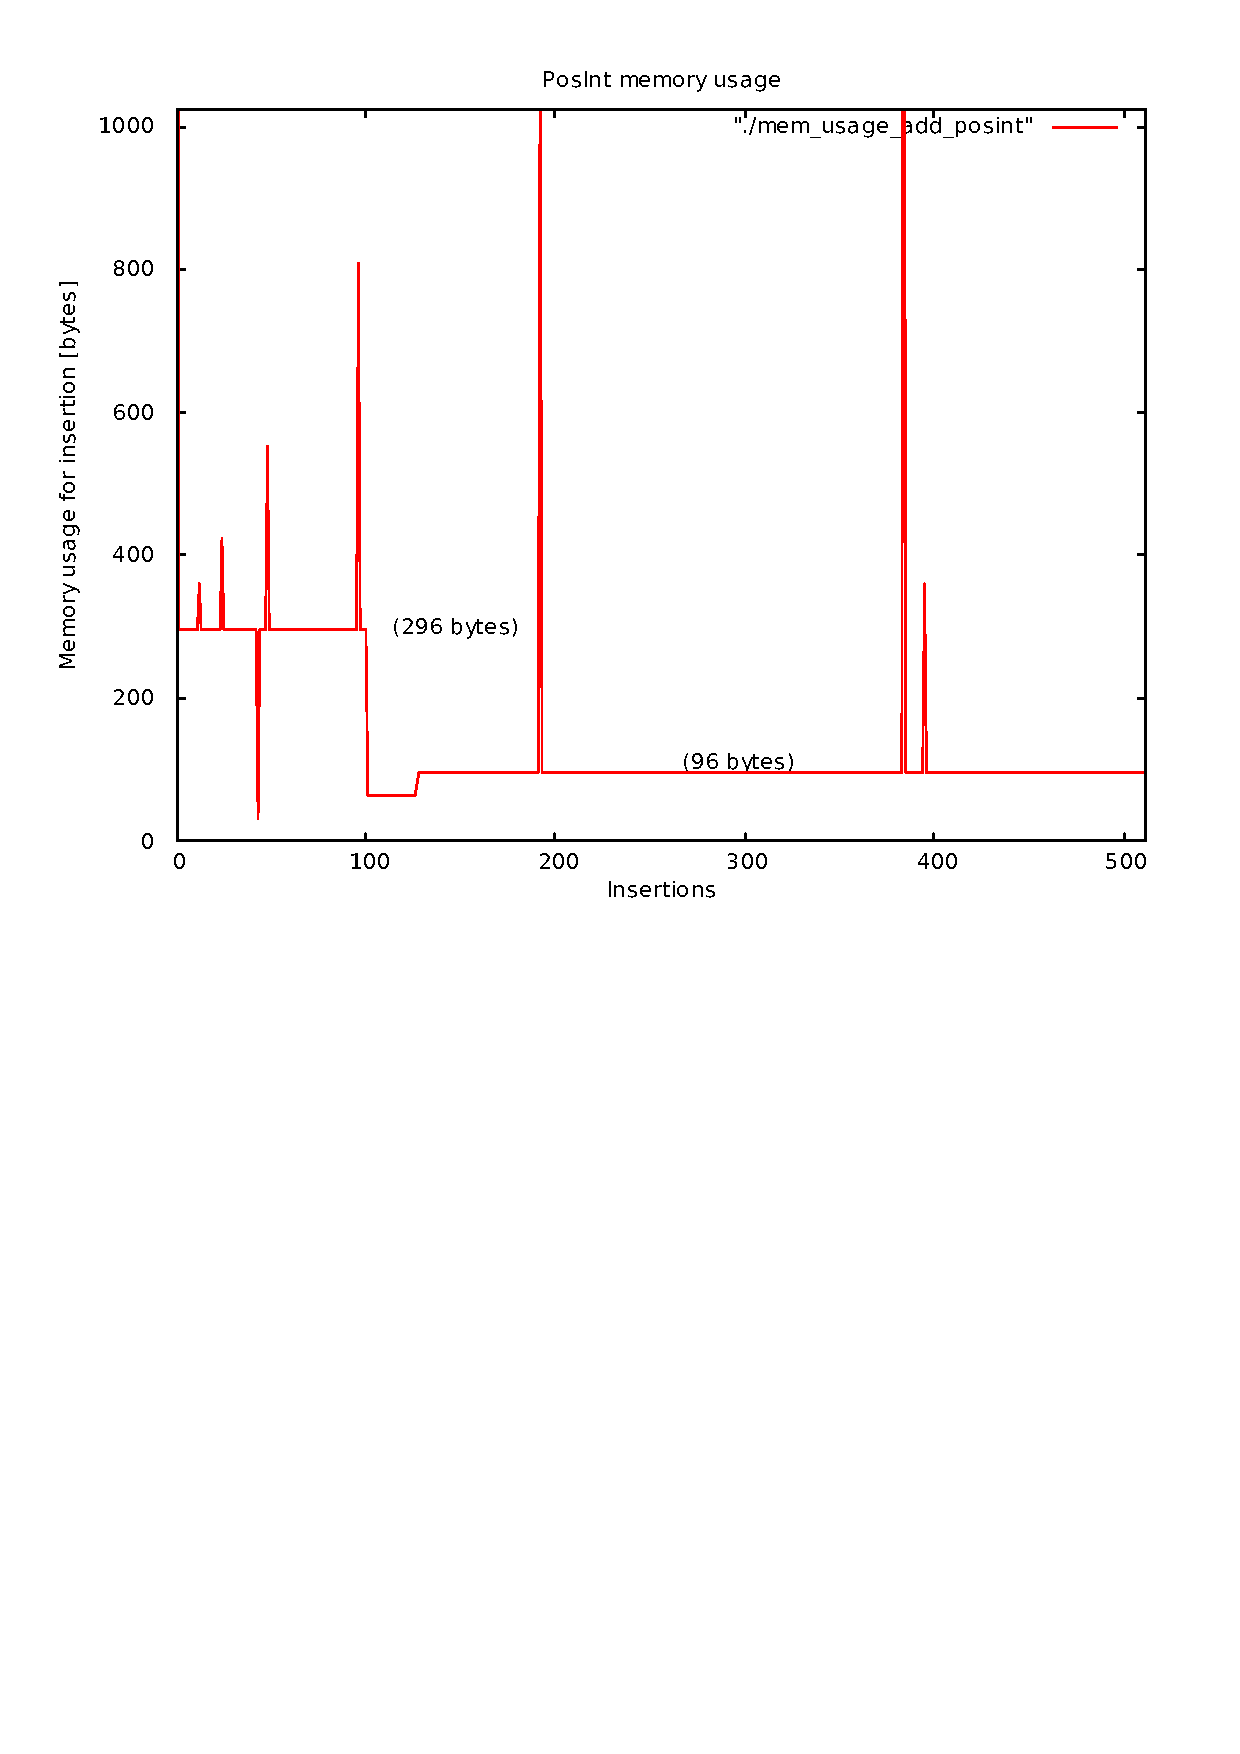
\includegraphics[width = 0.8\textwidth, trim = 0 15cm 0 0] {img/memoryConsumption_posint.pdf}
\caption{The memory usage}
\label{fig:memUsageInsertionPosInt}
\end{figure}


\subsubsection{Discussion}

Ideally, each insertion would take up the same amount of memory, but
figure \ref{fig:memUsageInsertionPosInt} suggests otherwise. The
very first insertion is shown to cost 49128 bytes. The excessive size
can be attributed to class loading, which is performed at the first
initialization of a given object. After the first insertion, the memory
usage for each inserted integer is 296 bytes, then dropping to 64
bytes after 100 insertions. At the 128th insertion, the memory usage
for each insertion increases to 96 bytes, and it stays at this level
for the rest of the insertions. It is, however, difficult to conclude
what causes these memory changes, at these exact points in time.

The spikes that are seen at insertion number 12, 24, 48, 96, 192 and
384 are related to the expansion of hash maps.

96 bytes for storing an integer is a significant memory overhead,
caused by storing the data in our Entry objects. It can be explained
by the many levels of wrapping of values into objects, that occurs
in EDMA. The diagram shown in figure \ref{fig:valueStorageOverhead}
shows the wrapping that occurs when storing an integer value in EDMA.

\begin{figure}[h!]
\centering
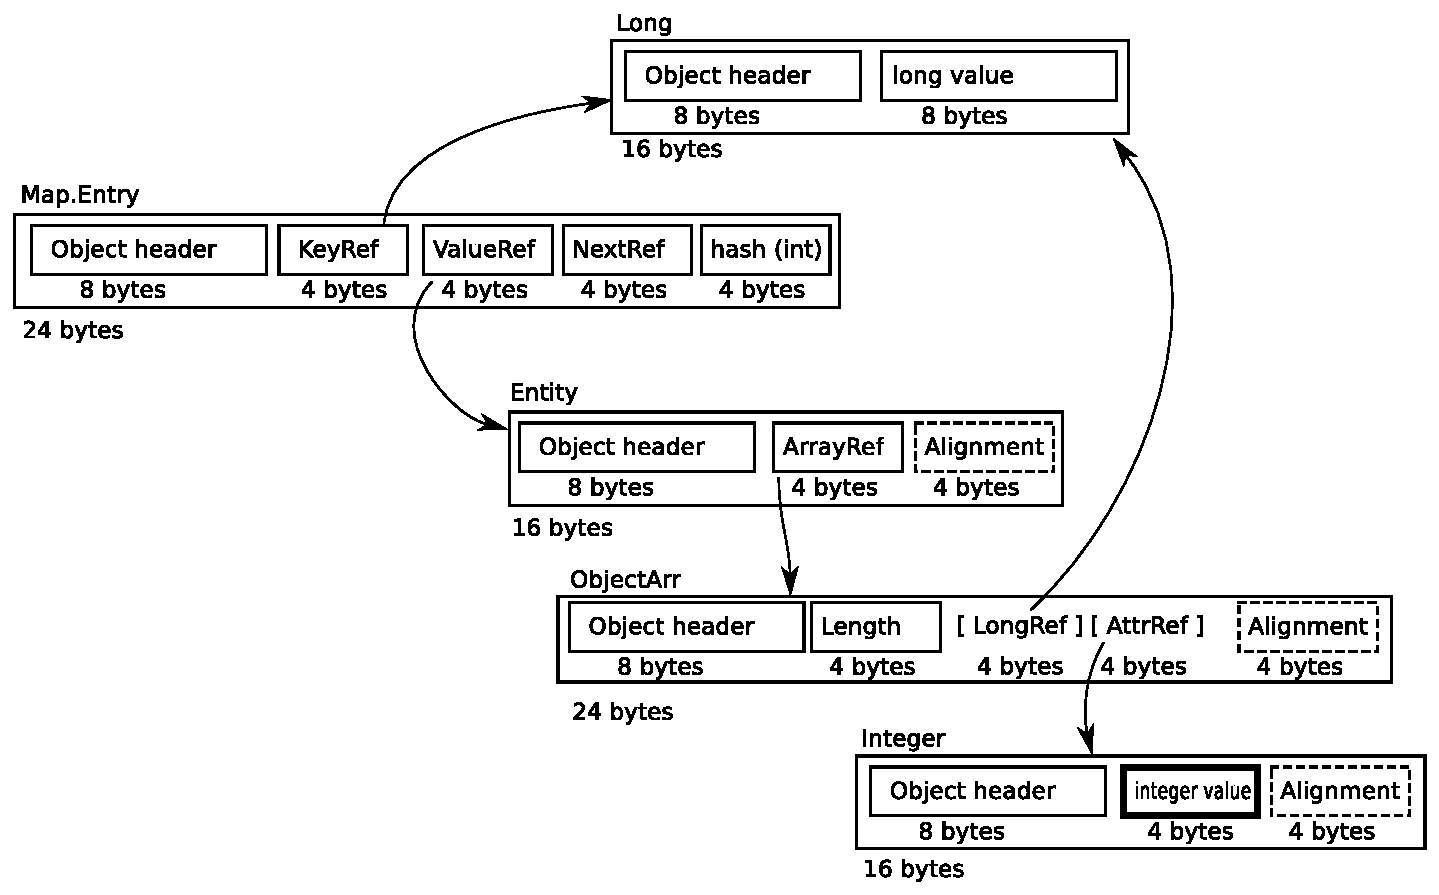
\includegraphics[width=\textwidth]{img/valueStorage.pdf}
\caption{This diagram shows the wrapping that occurs when storing data values in EDMA. A Map.Entry object holds a key reference and a value reference to the Entity object, wrapping the array containing the data value (the bold box).}
\label{fig:valueStorageOverhead}
\end{figure}

The diagram shows several contributions to the excessive memory use
-- object headers take up 8 or 16 bytes (on 32 bit and 64 bit platforms
respectively), and the JVM performs 8 byte alignment \cite{dieckmann1999study},
contributing to unnecessary allocation. This is further enhanced when
having many instances of small objects. The storage of the bold-boxed
integer in figure \ref{fig:valueStorageOverhead} adds up to a total
of 96 bytes, like the graph in figure \ref{fig:memUsageInsertionPosInt}
suggests.


\subsection{Data Insertion Response Time}

The response time for inserting data is measured in the following
procedure.
\begin{itemize}
\item Precondition: An empty data model instance must be started.
\item Flow of events:

\begin{enumerate}
\item Prepare an entity to insert.
\item Record the current time.
\item Insert the prepared entity.
\item Record the current time, and calculate the time difference.
\end{enumerate}
\end{itemize}
The reason for the entity value to be prepared before the time taking
starts, is that we want to measure only the response time of inserting
data -- not including creating the data values.


\subsubsection{Results}

Figure \ref{fig:insertionDvuResponse} shows the response time of
inserting entities. 

\begin{figure}[h!]
\centering
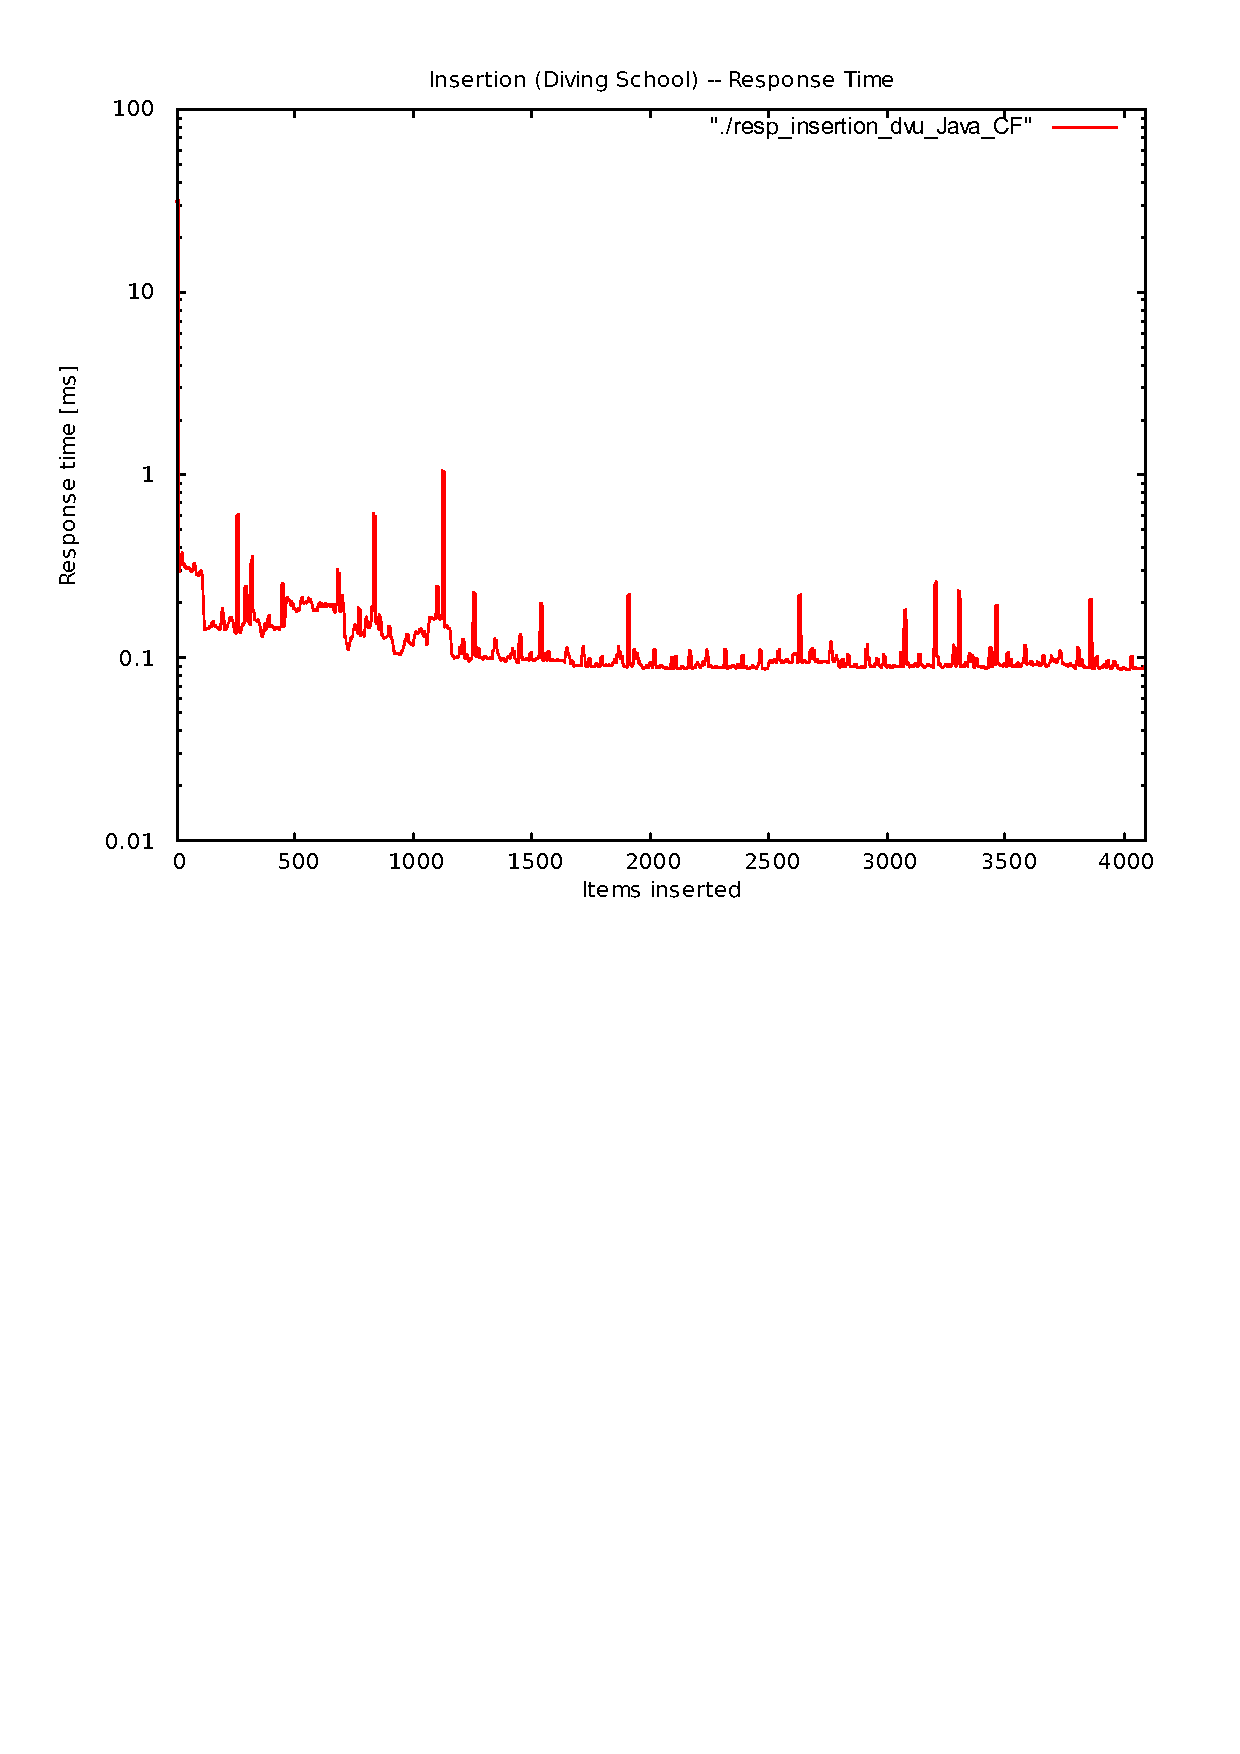
\includegraphics[width = 0.8\textwidth, trim = 0 15cm 0 1cm] {img/insertionDvuResponse.pdf}
\caption{This figure shows the response time of inserting new Person entities.}
\label{fig:insertionDvuResponse}
\end{figure}


\subsubsection{Discussion}

The response time for the very first insertion is rather high (31
ms), because it includes class loading. After classes have been loaded,
the response time drops to around 0.3 ms. After about 1200 insertions,
the response time finds a stable level at around 0.1 ms per insertion.


\subsection{Data Insertion Throughput}

In order to measure the throughput when inserting data, the following
procedure is executed.
\begin{itemize}
\item Precondition: An empty data model instance must be started.
\item Flow of events:

\begin{enumerate}
\item Create a number of worker threads, with the job of inserting a certain
number of entities.
\item Record the current time.
\item Start all the worker threads.
\item Join all the worker threads (wait for their finish.)
\item Record the current time, calculate the time difference and throughput.
\item Clear the data model instance -- remove all entities.
\item Increase the number of worker threads, and go back to step 1.
\end{enumerate}
\end{itemize}
The test has been run, inserting 32768 Person entities, divided between
the number of worker threads. 


\subsubsection{Results}

Figure \ref{fig:insertionDvuThroughput} shows the insertion throughput,
varied by the number of concurrent worker threads. It is seen that
the single-threaded throughput measure is at the lowest, running at
12 insertions/ms. Running with two threads increases the throughput
to 22 insertions/ms, and with four threads the throughput is 44. Running
with up to 100 threads, the throughput varies between 46 and 57 insertions/ms.

\begin{figure}[h!]
\centering
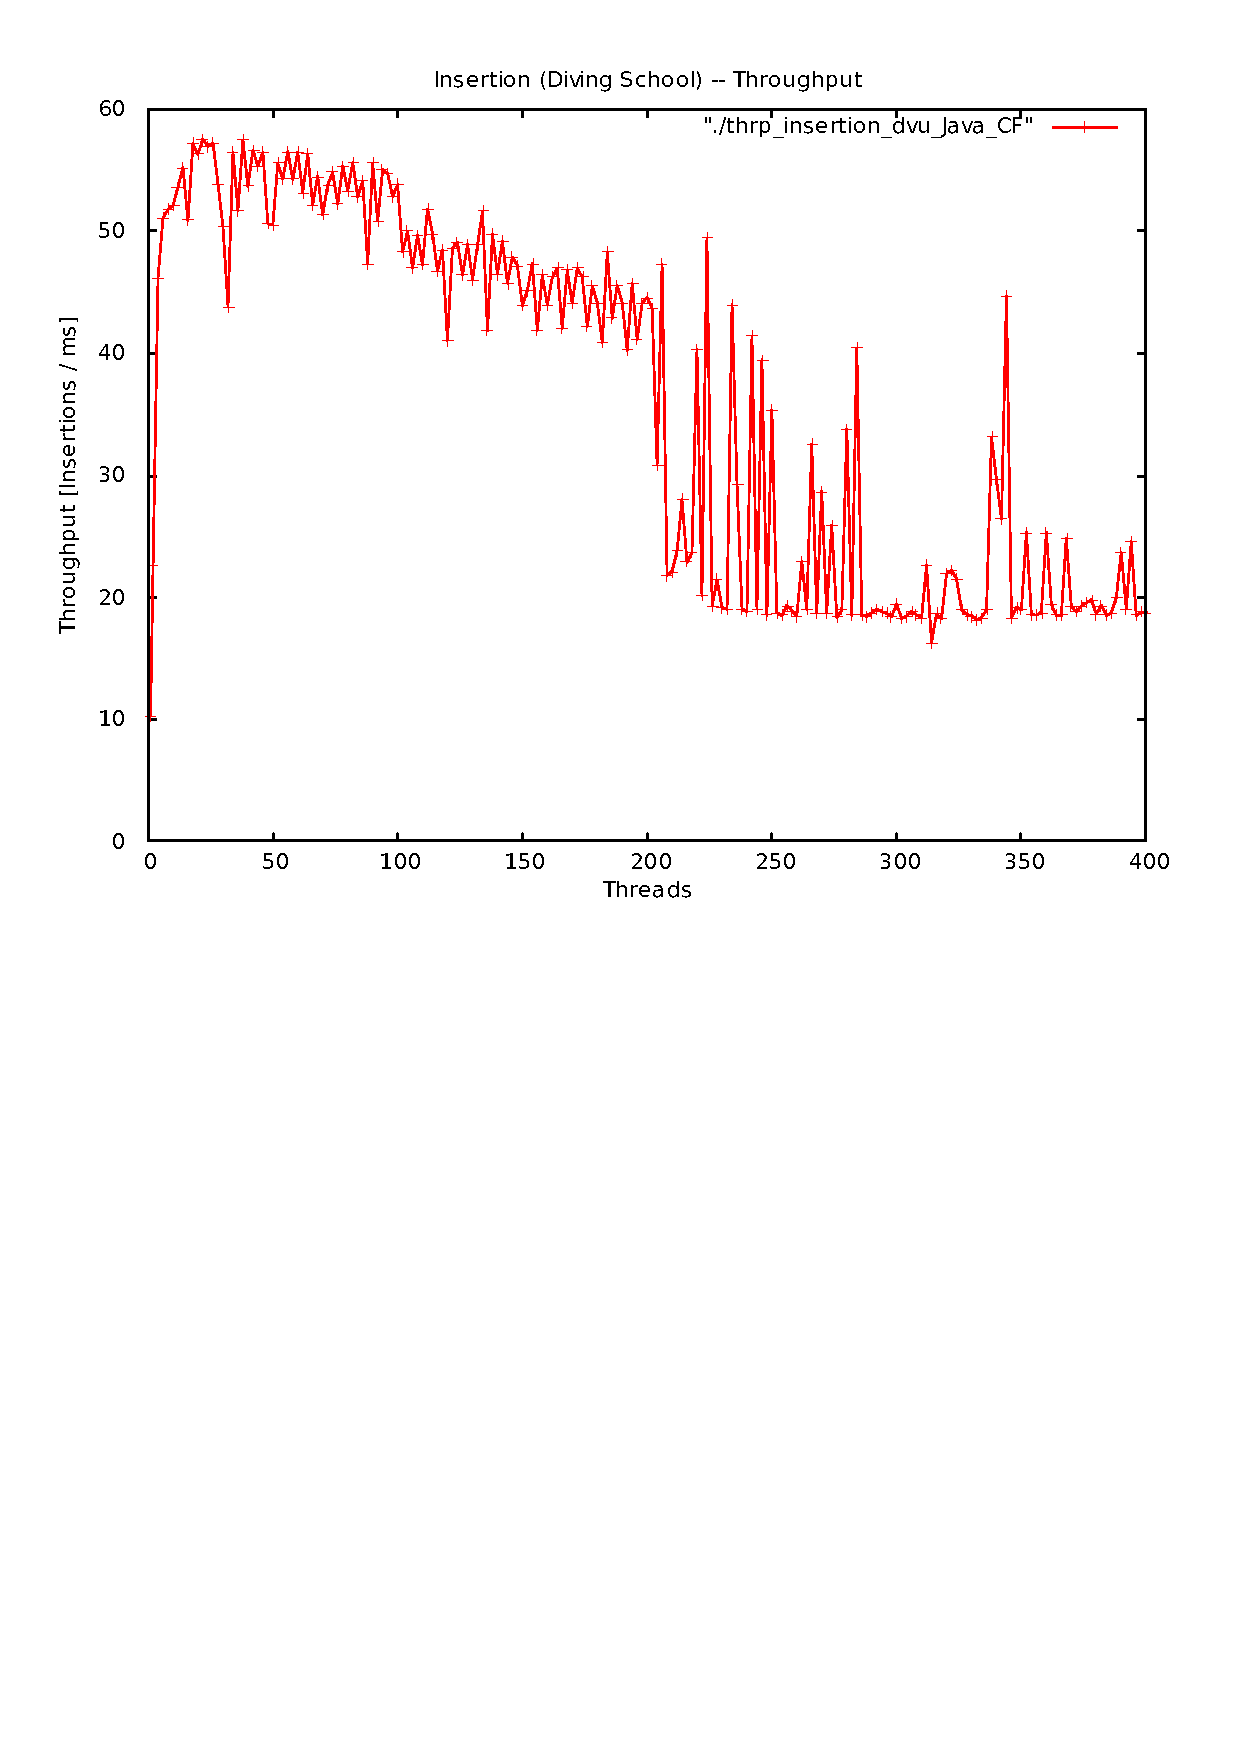
\includegraphics[width = 0.8\textwidth, trim = 0 15cm 0 1cm] {img/insertionDvuThroughput.pdf}
\caption{This figure shows the throughput (insertions per ms), as a function of the number of concurrent threads.}
\label{fig:insertionDvuThroughput}
\end{figure}Running with more than 100 threads shows a decreasing tendency in
the throughput. This might be because either the execution buffer,
or the persistence buffer, is occasionally full -- they are both set
to a maximum size of 100, in the current implementation. Using 200
or more threads, shows a drastic decrease in the throughput, because
both of the buffers are filled, causing blocking of the worker threads.
Here, the throughput falls to about the same level as when using 2
threads (around 20 insertions/ms.)


\subsubsection{Discussion}

It is not obvious, why the graph looks like it does. Going from one
to two threads doubles the throughput as expected, but we wouldn't
expect much more throughput by using more than two threads. A plausible
explanation would be the overhead that is involved in changing the
state of threads, by calling wait and notify. The two running units
in our two step pipeline utilize two synchronized buffers, causing
many calls to wait and notify. Using two threads, we keep the slowest
of the two execution units (often the persistence unit) busy However,
when using 3 or more threads, both the executor and the persist are
kept busy most of the time, causing fewer thread state changes. This
could explain why extra performance is gained using more than 2 threads.


\subsection{Data Retrieval Response Time}

In order to measure the response time of retrieving data, we insert
a large number of Person entities into a running data model instance.
We then search for persons, that we know have been put into the data
model instance.
\begin{itemize}
\item Precondition: A data model instance has been started, and 10000 Person
entities has been inserted. The first and last name of each Person
entity has additionally been stored in a list.
\item Flow of events:

\begin{enumerate}
\item Get a random first name and last name from the list of inserted names.
\item Record the current time.
\item Run the view that retrieves Persons from the chosen first name and
last name.
\item Record the current time, calculate the time difference, and go back
to step 1.
\end{enumerate}
\end{itemize}

\subsubsection{Results}

The response time when using two different indexes (a compare index
and an equals index) is shown in figure \ref{fig:retrievalDvuResponse}.

\begin{figure}[h!]
\centering
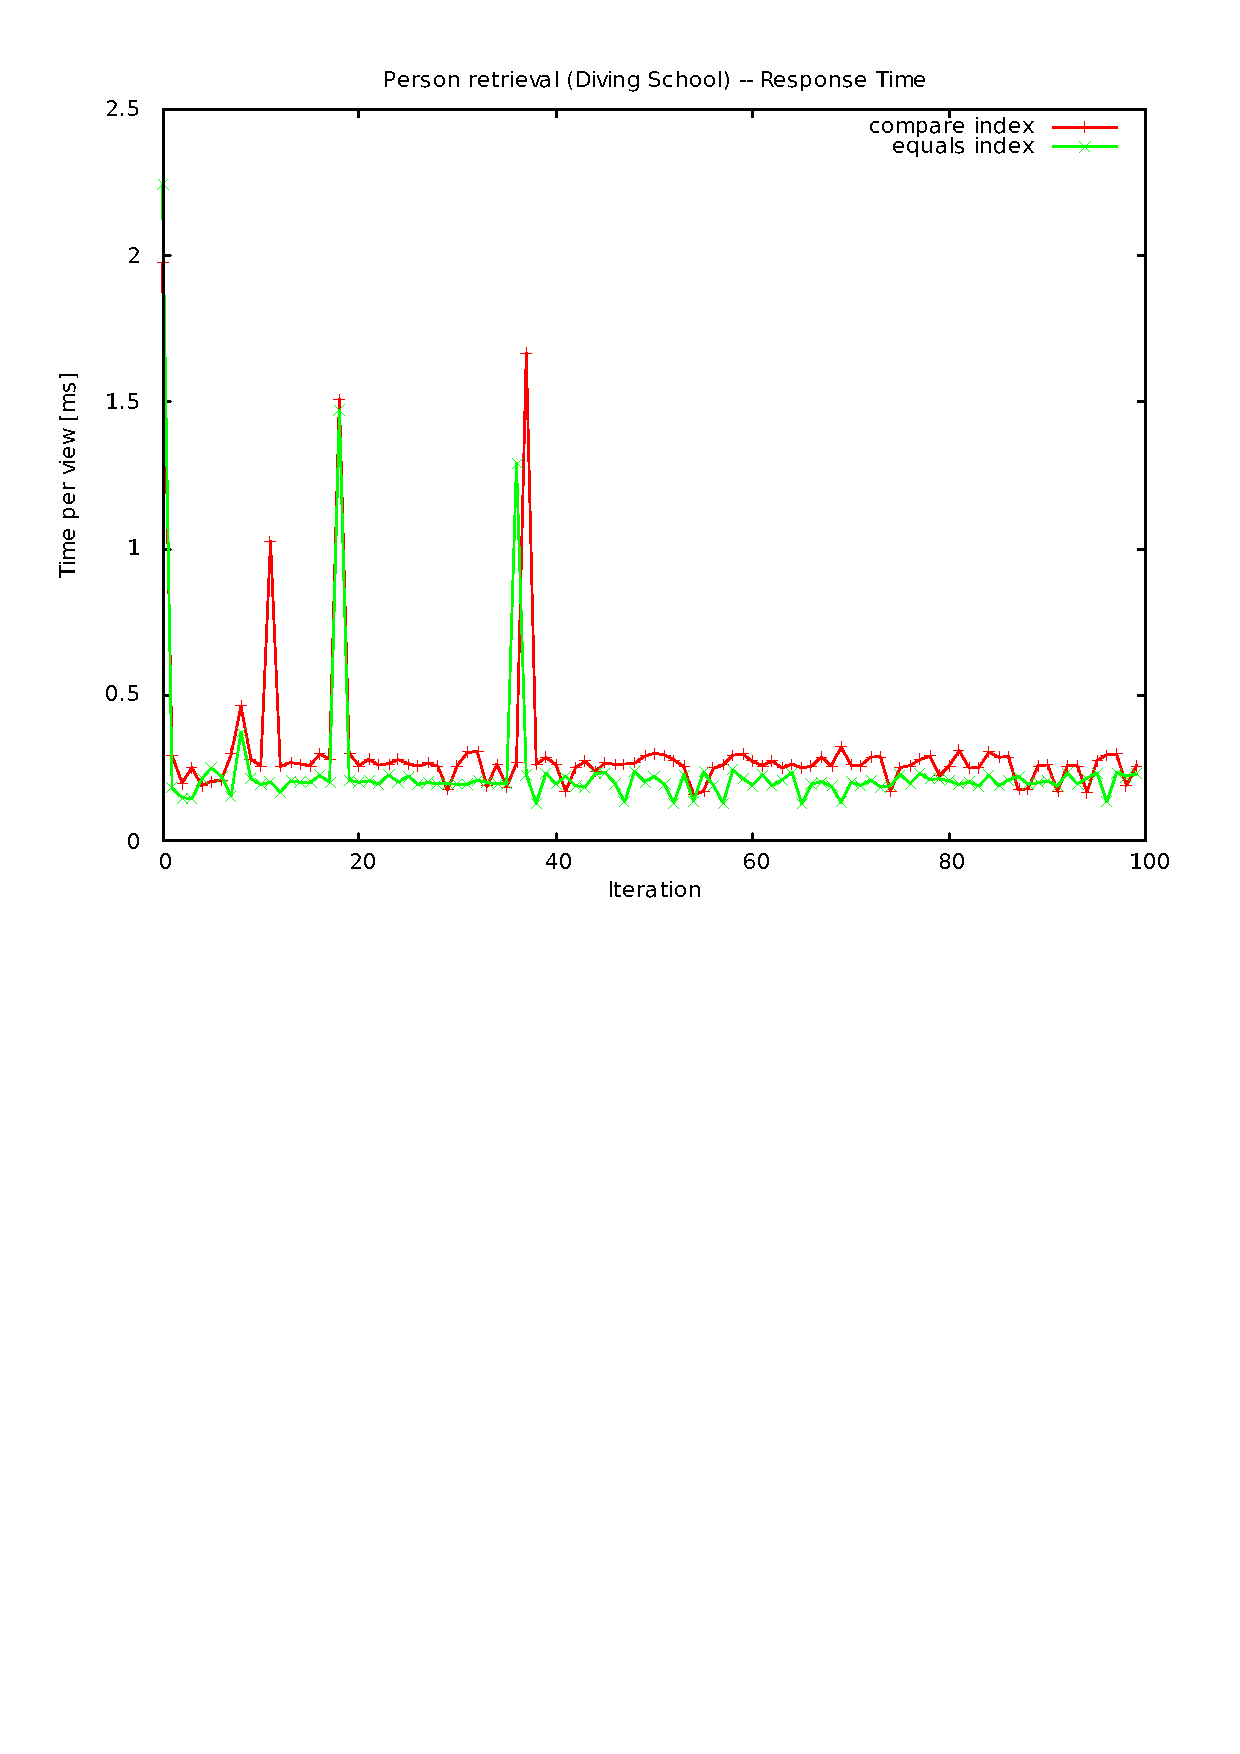
\includegraphics[width = 0.8\textwidth, trim = 0 15cm 0 1cm]{img/retrievalDvuResponse.pdf}
\caption{This figure shows the response time for searching for Persons with a randomly chosen name (guaranteed to find at least 1), using two different types of indexes.}
\label{fig:retrievalDvuResponse}
\end{figure}


\subsubsection{Discussion}

The response time lies around 0.16 ms to 0.30 ms when using the compare
index (which is based on a tree map), while the equals index (based
on a hash map) is slightly faster, ranging from 0.12 ms to 0.22 ms.


\subsection{Data Retrieval Throughput}

Measuring the throughput of retrieving data is done by creating a
variable amount of worker threads, each retrieving a Person from the
first name and last name.
\begin{itemize}
\item Preconditions: A data model instance is started, and 100.000 Person
entities has been inserted. The first and last name of each Person
entity has additionally been stored in a list.
\item Flow of events:

\begin{enumerate}
\item Run garbage collection and finalization.
\item Create a number of worker threads, each with the task of retrieving
a person from a first name and last name.
\item Record the current time.
\item Start all the worker threads.
\item Join all the worker threads.
\item Record the current time.
\item Calculate the throughput, as the number of views executed per millisecond.
\item Increase the number of worker threads, and go back to step 1.
\end{enumerate}
\end{itemize}
The worker threads together execute a total of one million views.


\subsubsection{Results}

The results for the throughput measuring can be seen in figure \ref{fig:retrievalDvuThroughput}.

\begin{figure}[h!]
\centering
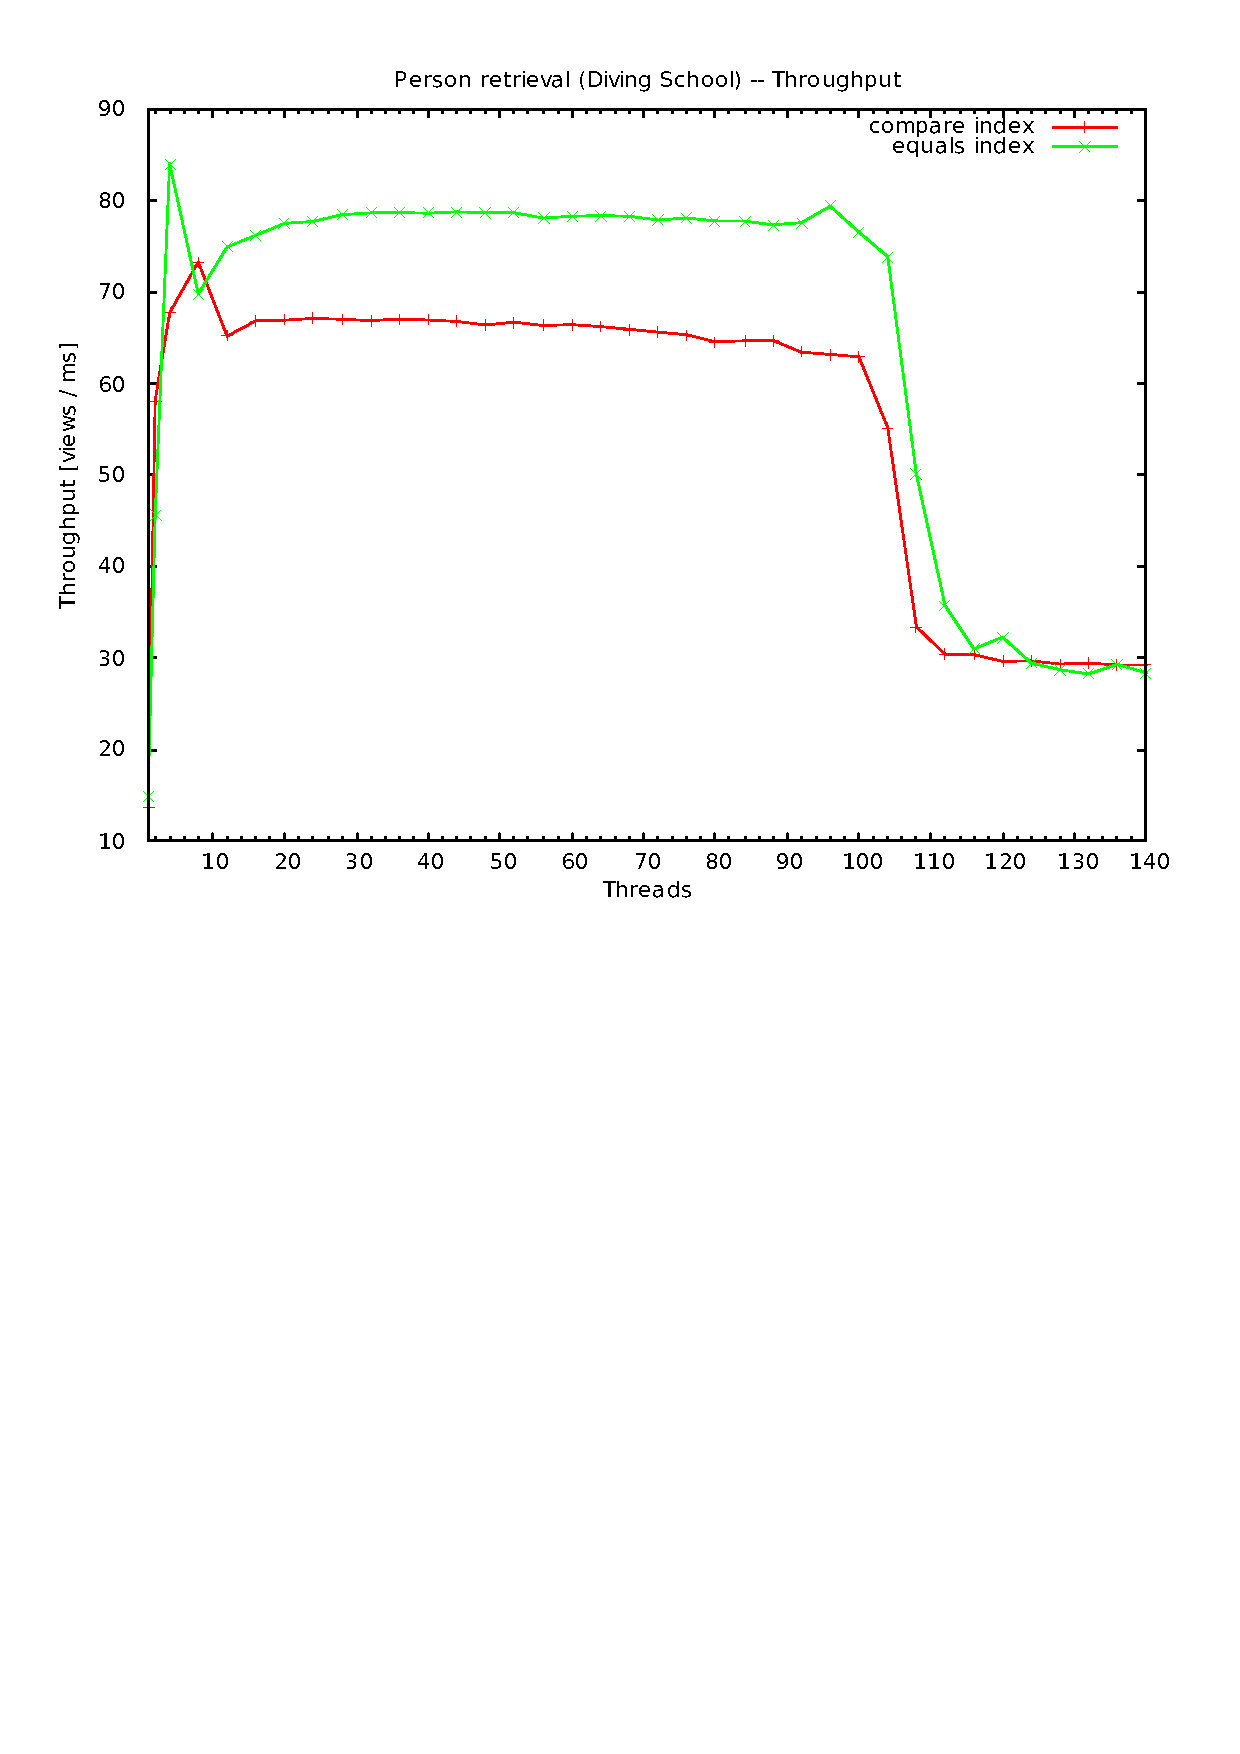
\includegraphics[width = 0.8\textwidth, trim = 0 15cm 0 1cm]{img/retrievalDvuThroughput.pdf}
\caption{This figure shows the throughput of having a number of threads searching for Persons with randomly chosen names (guaranteed at least one hit). Two different kinds of indexes are used, a compare index and an equals index.}
\label{fig:retrievalDvuThroughput}
\end{figure}

The x-axis shows the number of concurrent threads to perform the views,
and the y-axis shows the calculated number of persons that was retrieved
per millisecond.

Running with one thread gives a throughput of 13.75 views / ms with
the compare index, and 14.8 with the equal index. Increasing the number
of threads to 2 gives a compare index throughput of 58 views / ms,
while the equals index is 45 views / ms. The throughput stabilizes
at around 78 views / ms for the equals index, and 67 views / ms for
the compare index, as long as there are less than 100 worker threads.
Using more than 100 threads, the throughput drops to about 30 views
/ ms.


\subsubsection{Discussion}

The results show, as expected, that the equals index has a higher
throughput value than the compare index, and that running with multiple
threads has a great impact, compared to running with only one thread.
However, when the number of threads is higher than the size of the
execution buffer (here 100), the throughput drops to around 30 views
/ ms.


\subsection{Interleaved Actions and Views}

In order to see how the number of actions affects the total throughput,
when running interleaved actions and views, we run the following procedure.
\begin{itemize}
\item Precondition: A data model instance has been started, and 100.000
Person entities has been inserted.
\item Flow of events:

\begin{enumerate}
\item $p_{action}$, the probability of running an action instead of a view,
is set to 0.
\item While \emph{$p_{action}\leq1$}

\begin{enumerate}
\item 50 worker threads are created, with the task of running either an
action or a view in each iteration, depending on $p_{action}$.
\item The current time is recorded.
\item All the worker threads are started.
\item All the worker threads are joined.
\item The current time is recorded.
\item The total number of actions and views are determined.
\item The total throughput, the view throughput and the action throughput
is calculated.
\item $p_{action}$ is increased by 0.02.
\end{enumerate}
\end{enumerate}
\end{itemize}

\subsubsection{Results}

The result of running interleaved actions and views can be seen in
figure \ref{fig:interleavedActionsAndViewsThroughput}.

\begin{figure}[h!]
\centering
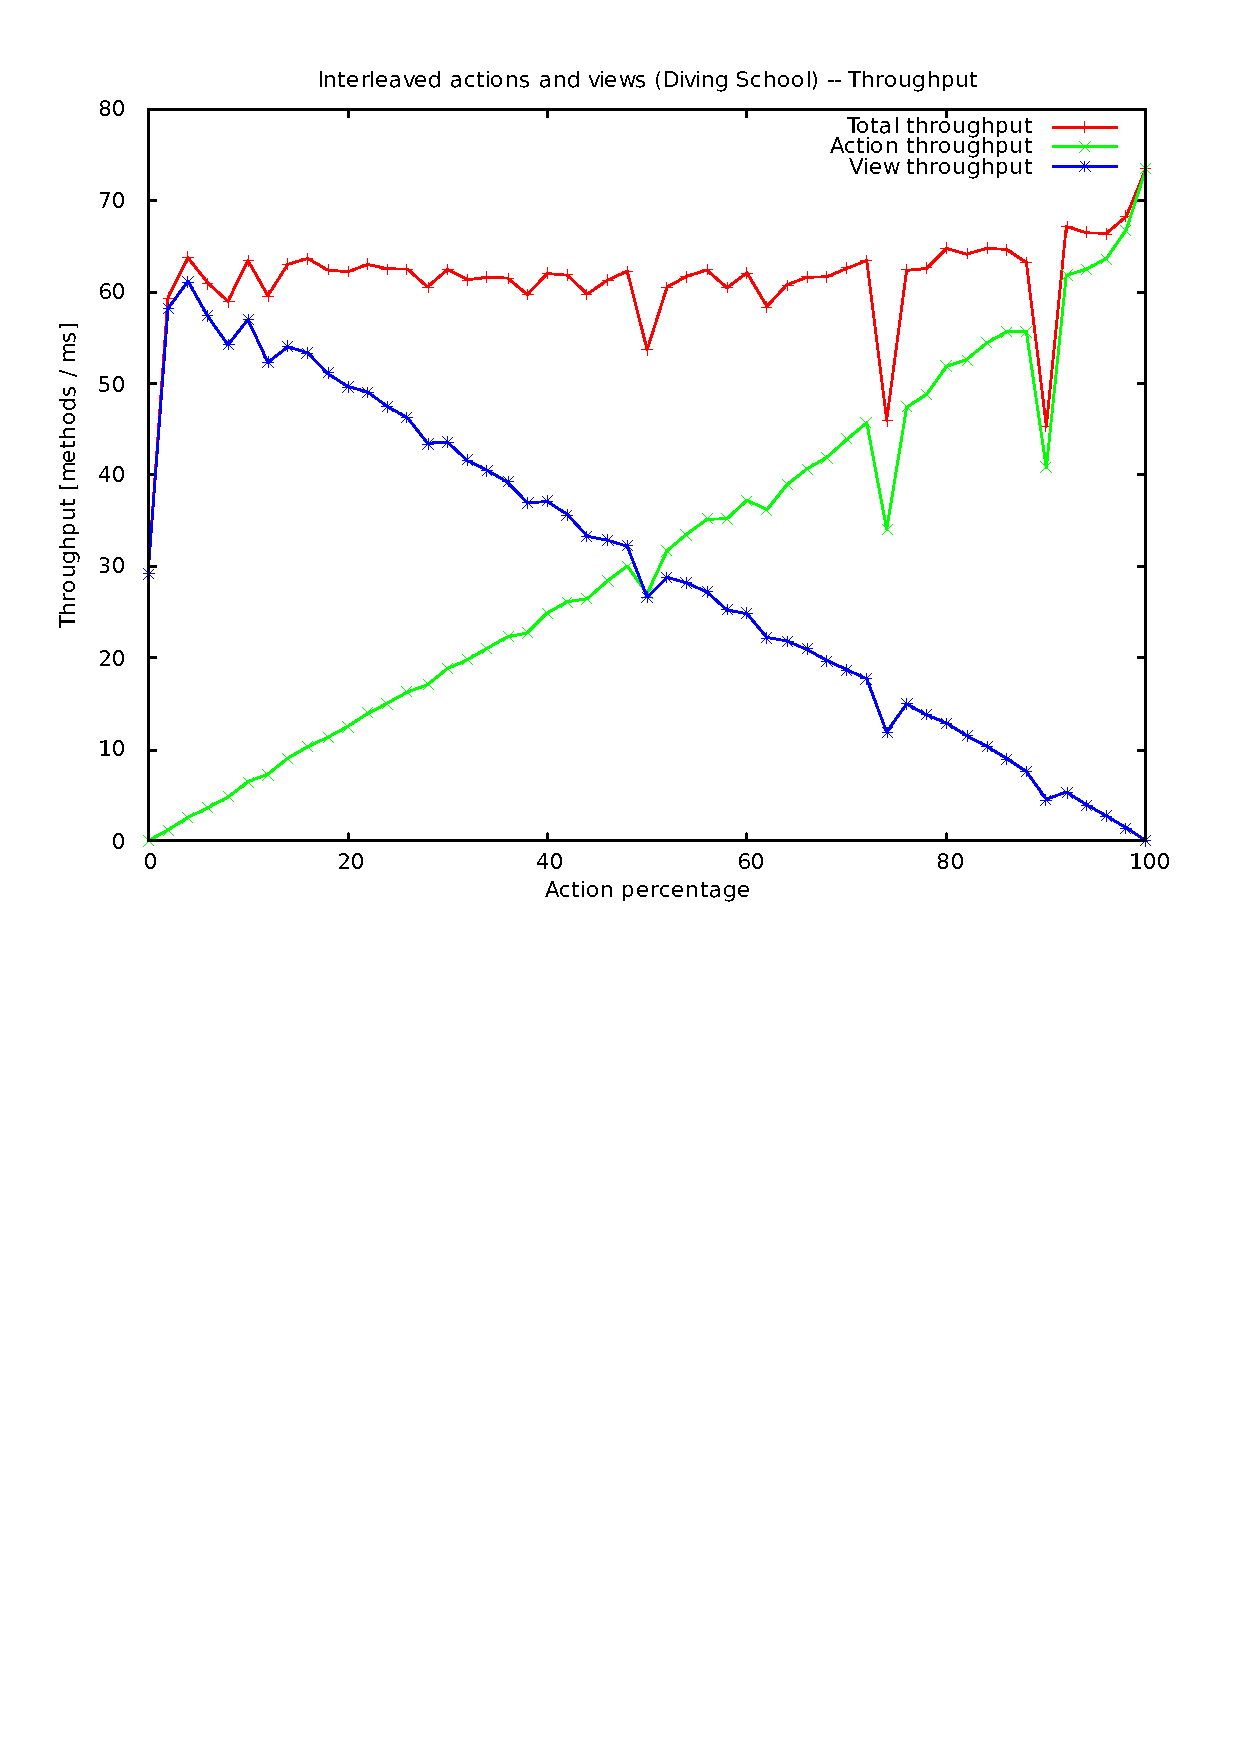
\includegraphics[width=0.8\textwidth, trim=0 15cm 0 1cm] {img/interleavedActionsAndViewsThroughput.pdf}
\caption{This graph shows the result of running interleaved actions and views. 50 worker threads are set to run concurrently. Each worker thread runs for a number of iterations, where each iteration can run either an action or a view, determined by the probability factor (the x-axis). The throughput is shown on the y-axis.}
\label{fig:interleavedActionsAndViewsThroughput}
\end{figure}


\subsubsection{Discussion}

The graph shown in figure \ref{fig:interleavedActionsAndViewsThroughput}
shows that the total throughput remains constant, even if the probability
of running actions increases. The action throughput seems almost directly
inverse to the view throughput, which is contrary to our expectations.
Since our runtime system is able to run multiple views concurrently,
but not actions, we would expect a dropping total throughput, when
increasing the number of actions run.


\subsection{Scalability}

Scalability denotes the possibilities of adding workload to the system.
Andre B. Bondi of Bell Labs proposes definitions of 6 different scalability
aspects in \cite{bondi2000characteristics}. According to Bondi, there
are at least the following aspects of scalability:
\begin{lyxlist}{00.00.0000}
\item [{Load~Scalability}] -- describes how well a system is able to function
gracefully at light, moderate or heavy load, i.e. mostly considering
variance in the number of users.
\item [{Space~Scalability}] -- describes how the memory requirements changes,
as the amount of data handled by a system changes. The system can
be considered spatially scalable, if the memory usage grows sublinearly
with the number of data items in question.
\item [{Space-Time~Scalability}] -- describes the ability for a system
to function gracefully, when the amount of data changes by orders
of magnitude.
\item [{Structural~Scalability}] -- describes whether a system uses data
structures or algorithms that naturally limit the amount of data that
can be contained or dealt with.
\item [{Distance~Scalability}] -- the ability for a system to operate
over short as well as long distances (considering issues such as reliability
at drop-outs, timing issues, noise, etc.)
\item [{Speed/Distance~Scalability}] -- the ability for a system to operate
at high speed over short as well as long distances.
\end{lyxlist}
Throughout the project, some of these scalability aspects has been
prioritized higher than others. In the beginning of developing the
EDMA system, although not formally stated anywhere, it was the thought
that it should be able to serve small businesses with ``thousands''
of users (<10000). 


\subsubsection{Load Scalability}

The load scalability mainly depends on the execution of actions and
views, together with the persistence. According to Bondi, load scalability
can be improved by not having unproductive execution cycles in the
program, avoiding busy waiting, and allow parallel execution where
possible. As explained in the section about the transaction execution,
EDMA is able to execute multiple views at the same time. However,
only one action can be executed at the time, which puts a boundary
on the load scalability. However, even if only one action can be executed
at the time, heavy load will have the system continue gracefully,
until a certain degree, determined by the maximum size of the execution
buffer and the persistence buffer. When these are both filled, throughput
decreases drastically, as shown in the test of data insertion throughput.


\subsubsection{Space Scalability}

The space scalability depends on how data is stored in the runtime
system, and how it is persisted on the disk.

In the runtime system, data is held in the memory, in the kind stores.
The kind stores hold all data entities in maps, with an ID as key
(as a long), and an Entity object as value. The Entity contains an
Object array, holding the actual attribute values. However, the value
domain system uses instance control, guaranteeing that two equal values
will only be instantiated once in the memory. Therefore, the entities
that are kept by the kind store may reuse each others' values. However,
the kind store still has to hold separate Entity objects for each
entity, making it linearly growing with the amount of data. This makes
the system less scalable as seen from the spatial aspect. The upper
bound for the amount of data is decided by the choice of either using
Java maps, or maps from the JDBM3 library (the user chooses this upon
instantiation of the data model.) If the former is used, the upper
bound is determined by the amount of RAM that is available to the
Java Virtual Machine. If the latter is used, the upper bound is determined
by the disk size.


\subsubsection{Space-Time scalability}

With respect to data search, EDMA uses tree maps for compare-indexes
and hash maps for equal-indexes, making it efficient. If the user
instead uses a custom made filter to search for data of a certain
kind, data is traversed linearly, hurting the space-time scalability.
Therefore, the user should be encouraged to use indexes as much as
possible, and applying custom filters as late in the search process
as possible.


\subsubsection{Structural scalability}

Naturally, there are limits for how much data can be stored. If regular
Java maps are used for storing the runtime data, the amount of RAM
accessible is a limit for the data amount, and the file system is
a limit for the log file size. 

From the user's point of view, some aspects of the EDMA system are
structurally scalable, while others are not. There are some logical
problems in changing a data model, after it has been taken into use
-- for example:
\begin{itemize}
\item If a kind is removed, what should be done when the data model tries
to load the log file, where the kind existed?
\item If non-optional attributes are added to a kind, or a new kind with
non-optional attributes is added, what should be the values of the
new attributes? When the log file is loaded, how can kind entities
be created, if there are no stored values for the newly added attributes?
\item What should be done if a kind or an attribute is renamed?
\end{itemize}
Some of these problems can be solved by having more interaction with
the user -- for example, in the case of renaming an element, the user
could explicitly tell EDMA the old name and the new name of the element,
upon instantiation. In the case of newly added attributes, the user
could either manually or automatically supply the missing data, possibly
adding null-data or temporary ``dummy'' data (e.g. 00000000 for
phone number.)

In this project, we haven't taken into account that the user should
be able to change the data model after it has been taken into use.
However, because of it's structure, the user is able to make the following
changes to a data model, after it has been taken into use (i.e. data
has been stored in the log file):
\begin{itemize}
\item Adding kinds (after the last kind in the data model in the data model
definition)
\item Adding optional attributes to kinds
\item Adding relations (after the last relation in the data model definition)
\item Adding actions and views
\item Adding indexes to existing kinds and relations
\end{itemize}
The reason to only be able to be added ``in the end'', is that the
runtime system uses the sequential order of the kind (0, 1, 2, ...)
in the definition file, rather than the kind name. Adding a kind in
the top, will therefore push all the other kinds one step forward,
which will invalidate the log file. 

The following is not possible without substantial changes to the system:
\begin{itemize}
\item Removing or renaming kinds, attributes, relations, actions or views
(renaming or removing actions or views does not break anything in
the runtime system directly, but will break the user's code)
\item Adding non-optional attributes to kinds\end{itemize}

